%%%%%%%%%%%%%%%%%%%%%%%%%%%%%%%%%%%%%%%%%%%%%%%%%%%%%%%%%%%%%%%%%%%%%%%%%%%%
% To the extent possible under law, the person who associated CC0 with     %
% this document has waived all copyright and related or neighboring rights %
% to this document.                                                        %
%                                                                          %
% You should have received a copy of the CC0 legalcode along with this     %
% work.  If not, see <http://creativecommons.org/publicdomain/zero/1.0/>.  %
%%%%%%%%%%%%%%%%%%%%%%%%%%%%%%%%%%%%%%%%%%%%%%%%%%%%%%%%%%%%%%%%%%%%%%%%%%%%

\documentclass{article}
\usepackage[margin=0.5in]{geometry}
\usepackage[utf8]{inputenc}
\usepackage{amsmath}
\usepackage{graphicx}
\usepackage{float}
\usepackage{multicol}
\usepackage{lscape}
\usepackage{xparse}
\usepackage{colonequals}
\usepackage{ragged2e}
\usepackage{titlesec}
\usepackage{tikz}

\setlength{\parindent}{0cm}
\parskip=7pt plus 1pt
\pagenumbering{gobble}
\titlespacing\section{0pt}{5pt plus 4pt minus 2pt}{0pt plus 2pt minus 2pt}
\titlespacing\subsection{0pt}{5pt plus 4pt minus 2pt}{0pt plus 2pt minus 2pt}

\graphicspath{{./img/}}

\begin{document}
    \begin{landscape}
        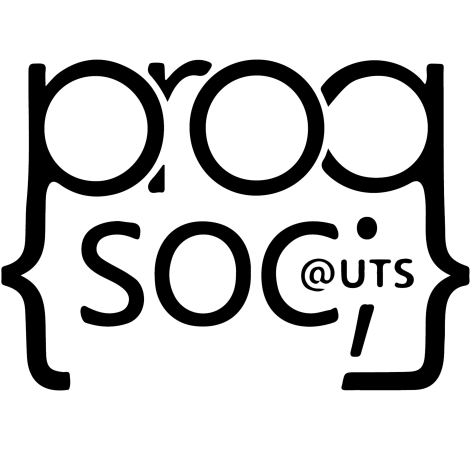
\includegraphics[height=1.3cm]{progsoc.png}

        \vspace{-1.3cm}

        \begin{center}
            \begin{LARGE}
                \textbf{Shaders Cheatsheet}
            \end{LARGE}
        \end{center}
        \begin{multicols}{3}

            \section{GLSL Boilerplate}
            \subsection{Vertex Shader}
            \begin{verbatim}
#version 300 es
in float someAttribute;
out vec2 someVarying;

void main() {
    someVarying = vec2(1.);
    gl_Position = vec4(1.);
}
            \end{verbatim}

            \subsection{Fragment Shader}
            \begin{verbatim}
#version 300 es
precision highp float;
out vec4 FragColor;
in vec2 someVarying;

void main() {
    FragColor = vec4(1.);
}
            \end{verbatim}

            \section{GLSL Functions}
            \begin{small}
                \begin{tabular}{l l}
                    \texttt{mix(a, b, amount)} & Interpolate scalars or vectors \\
                    \texttt{pow(x, y)} & $x^y$ \\
                    \texttt{clamp(x, min, max)} & Clamp \texttt{x} to \texttt{min} and \texttt{max} \\
                    \texttt{dot(u, v)} & $\vec u \cdot \vec v$ \\
                    \texttt{cross(u, v)} & $\vec u \times \vec v$ \\
                    \texttt{normalize(v)} & Normalise \texttt{v} to length 1 \\
                    \texttt{length(v)} & Length of \texttt{v} \\
                    \texttt{reflect(I, N)} & Reflect \texttt{I} about \texttt{N} \\
                    \texttt{refract(I, N, eta)} & \texttt{reflect} with index ratio \texttt{eta} \\
                    \texttt{step(edge, x)} & 1 if \texttt{x} is greater than \texttt{edge} \\
                    \texttt{smoothstep(e0, e1, x)} & Smooth interpolation \\
                    \texttt{matrixCompMult(A, B)} & Component-wise multiplication \\
                    \texttt{texture(sampler, uv)} & Sample a texture \\
                    \texttt{fract(x)} & Fratcional part of \texttt{x} \\
                \end{tabular}
            \end{small}
            \section{Glossary}
            \begin{tabular}
                {l l}
                Invocation & A single execution instance of a shader \\
                UV & Texture coordinates \\
                Normal & Vector perpendicular to surface \\
                Varying & Interpolated value between vertices \\
                Attribute & Per-vertex data \\
                Primitive & Line or triangle \\
                Fragment & Potential pixel in primitive \\
                Frame Buffer & Texture to render to \\
                Texel & Pixel in texture \\
                Blur Kernel & Offsets and weights for blurring \\
                $n^{\mp}$ & $n$ clamped to $[0, 1]$ \\
                $n^+$ & $n$ clamped to $[0, \infty]$ \\
            \end{tabular}

            \section{Lighting}
            \subsection{Phong}
            \begin{tabular}{l l}
                $I = I_a + I_d + I_s$ & Total intensity \\
                $I_d = (-\vec L \cdot \vec N)^{\mp}$ & Lambertian Diffuse intensity \\
                $R = 2(\vec L \cdot \vec N)\vec N - \vec L$ & Reflection vector \\
                $I_s = ((\vec R \cdot \vec V)^{\mp})^{\text{size}}$ & Specular intensity \\
            \end{tabular}

            \subsection{Fresnel}
            \begin{tabular}{l l}
                $F_0 + (1 - F_0)(1 - (\vec V \cdot \vec N)^+)^5$ & Schlick Fresnel \\
                $F_0 = \left(\frac{n_1 - n_2}{n_1 + n_2}\right)^2$ & Fresnel factor \\
            \end{tabular}
            \section{Techniques}
            \begin{itemize}
                \item \RaggedRight Shadow Mapping: \texttt{shadow = texture( shadowMap, shadowProj.xy).r - bias < shadowProj.z }
                \item Normal Mapping: \texttt{normal += normalize( texture(normalMap, uv) * 2.0 - 1.0)}
                \item Blur: Average surrounding pixels. Use Poisson disk for better results
                \item Random: Use hash function on UV and time
                \item Gamma Correction: \texttt{colour = pow(colour, vec3(1.0/gamma))}
                \item White Balance: \texttt{colour *= someColour.rgb}
                \item Skybox Reflection: \texttt{colour = mix(colour, texture(skybox, reflect(V, N)).rgb, reflectance * fresnel)}
            \end{itemize}

            \section{Clip Space}
            \begin{tabular}{l l}
                $(x/w, y/w)$ & Normalized Device Coordinates \\
                $z/w & Depth/Distance to camera \\
            \end{tabular}
            \section{Homogeneous Coordinates}
            $$
            \text{out}
            =
            \begin{bmatrix}
                x/w \\
                y/w \\
                z/w \\
            \end{bmatrix}
            $$
            \subsection{Transformations}
            \begin{small}
                \begin{tabular}{l l}
                    Translation & {
                    $$
                    \begin{bmatrix}
                        1 & 0 & 0 & x \\
                        0 & 1 & 0 & y \\
                        0 & 0 & 1 & z \\
                        0 & 0 & 0 & 1 \\
                    \end{bmatrix}
                    $$
                    } \\
                    Scale & {
                    $$
                    \begin{bmatrix}
                        x & 0 & 0 & 0 \\
                        0 & y & 0 & 0 \\
                        0 & 0 & z & 0 \\
                        0 & 0 & 0 & 1 \\
                    \end{bmatrix}
                    $$
                    } \\
                    Rotation (quaternion) & {
                    } \\
                \end{tabular}
                $$
                \begin{bmatrix}
                    1 - 2(y^2 + z^2) & 2(xy - zw )& 2(xz + yw) & 0 \\
                    2(xy + zw) & 1 - 2(x^2 - z^2) & 2(yz - xw) & 0 \\
                    2(xz - yw) & 2(yz + xw) & 1 - 2(x^2 - y^2) & 0 \\
                    0 & 0 & 0 & 1 \\
                \end{bmatrix}$$
                where $w = \cos(\theta/2)$ and $x, y, z = \sin(\theta/2)\vec v$ and $\vec v$ is the axis of rotation
            \end{small}
        \end{multicols}
    \end{landscape}
\end{document}
